\newpage

\thispagestyle{empty}

\chapter{Introduction}

	\hspace{15pt}Nowadays robots are not these futuristic and weird shaped machines as they were in the early 2000s American films. They are part of our life, and they make our days easier, more productive, and safer. It is pretty hard to define, what makes a robot, but we have some points which are true for all of them. First of all, we want to clarify, that our documentation will not say anything about software robots, we leave this topic to the IT security experts. The most important thing about machine robots is that they are programmable, and according to this program, it can make manipulations automatically. They can have external controller inputs, or they can have an embedded control. \cite{robotics2}

%Robotika alapjairól pár dolog, mit nevezünk robotnak, miért ezt nevezzük robotnak.

%1 oldal

%miért jók a robotok nekünk?

%hol tart jelenleg a robotika ilyen szempontból

%hol tart ezen belül ez manipulátor robot programozás
%mire használják őket

	\section{History of robots}

		\hspace{15pt}Robots have their roots from the ancient ages, these cultures wanted to make automated devices for entertainment purposes, but mankind only had the proper materials and methods from the industrial ages, and in these ages they wanted to use robots in the industry to make the production cheaper and faster. As we reached the modern ages, engineers and inventors introduced automatic, remote controlled, and wirelessly remote controlled robots too.	\cite{robotics1}
		
		\begin{figure}[H]
			\centering
			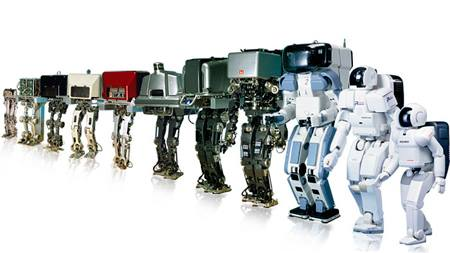
\includegraphics[width=\textwidth]{./images/history_of_robots}
			\caption{History of robots}
		\end{figure}


		The word robot, comes from the Czech language, and it means “forced labor”. In its modern form it has been firstly used by Karel Capek’s play in 1920. The science of robotics is the engineering field which deals with the design, construction and operation of robots. The word of robotics has been introduced in Isaac Asimov’s Sci-Fi “Runaround” in 1942. In his books Asimov has written down the three laws of robotics. These are the following: \cite{robotics1}

		\begin{enumerate}
			\item $"$A robot may not injure a human being, or, through inaction, allow a human being to come to harm.$"$ \\
			\item $"$A robot must obey the orders given it by human beings except where such orders would conflict with the First Law.$"$ \\
			\item $"$A robot must protect its own existence as long as such protection does not conflict with the First or Second Law.$"$ \\
		\end{enumerate} 

	\section{Modern robots}

		\hspace{15pt}In every modern factory you can see robots. Robotic arms which assemble whole cars, robot trains which transport products to the warehouse, industry 4.0 is not the future, we live in it. 

		Why are robots good for mankind? They can make monotonous processes all day long without a lunch or a cigarette break. They can be used in hazardous areas without any health risks. To cut a long story short, they make everything more productive, safer, quicker. Their designers should be aware that they have to help humans work, not to take all of their work to make human workers useless.

		According to industry 4.0 the separate robots and other machines are in a huge common network, and they synchronise their works, utilize the resources to reach the optimum. \cite{robotics2}

		\subsection{Types of modern robots}

			\begin{itemize}
				\item Mobile robots 
				\item Industrial (manipulator) robots 
				\item Service robots 
				\item Educational robots 
				\item Modular robots 
				\item Collaborative robots 
			\end{itemize}
			
			\subsubsection{Industrial (manipulator) robots}
			
				\hspace{15pt}Industrial robots are used for manufacturing, they are programmable and automated. They can move on two or more axes, but they are not able to change their physical position.
						
		\begin{figure}[H]
			\centering
			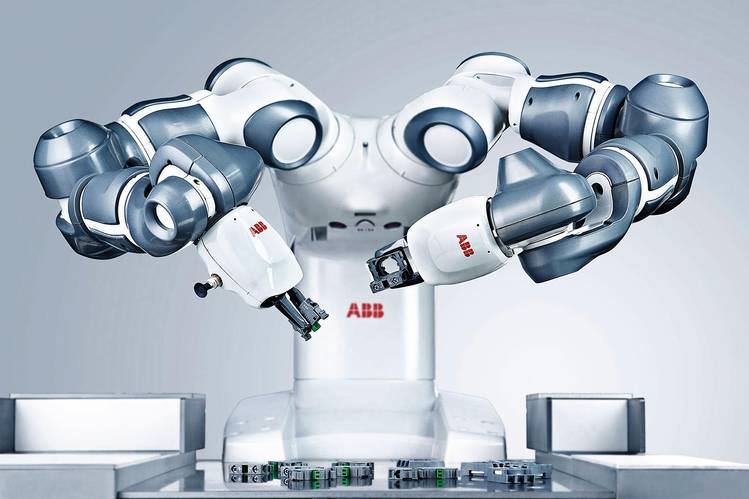
\includegraphics[width=\textwidth]{./images/manipulator}
			\caption{Manipulator robot}
		\end{figure}
				
				Their fundamental is the same, this structure has to be able to move a specific tool to the certain position, and hold it there until the manipulator finished its work. This manipulator can do welding, painting, screwing, lifting, etc. \cite{robotics2}

